In this chapter, we will introduce the general concepts and techniques behind Natural Language Processing. We will cover all the necessary steps for extracting meaningful topics from texts. % Finally, a brief discussion about machine learning for forecasting time series.


\section{Natural Language Processing}

	% Introdução geral sobre NLP

	\subsection{Text Processing Techniques}
	
	The key task to several machine learning problems consist in make a good data processing before applying any model. A clean data set can allow a model to increase its performance in the learning process, making a better identification in the patterns present in the variables. Hence, in the next sections, it will be discussed a few techniques to clear the text and prepare it for ML algorithms.
	
	\subsubsection{Normalization}
	%https://www.kdnuggets.com/2017/12/general-approach-preprocessing-text-data.html
	
	There is no right way to normalize text, this process has it is really important to put all text in the same level. A normalization process has a series of steps to be followed sequentially, all of then can be seen as 4 big tasks: stemming, lemmatization, stop words removal and everything else.
	
	\begin{enumerate}
		\item Stemming: Is the process of reduce inflected words to a primitive form, the stem. This method is able to remove the word's affixes to capture its base meaning, and still reducing the number of variations to save memory space. Figure \ref{fig:stemming} shows how some inflections for ``connect'' can be converted to its root form.
		
		\begin{figure}[h!]
			\centering
			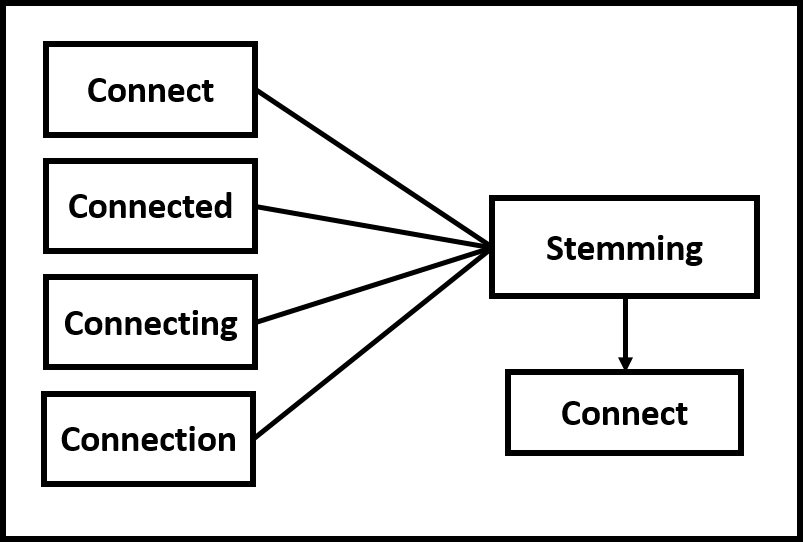
\includegraphics[width=0.45\linewidth]{01.Chapters/02.Background/stemming}
			\caption{Stemming process for ``connect'' variations \cite{vijayarani2015preprocessing}.}
			\label{fig:stemming}
		\end{figure}
		
		% stemming algorithms
		
		\item Lemmatization: similar to stemming, this step also reduce words to some primitive form, but with a little improvement. Lemmatization can returns the words to his dictionary form, based on its part of speech context. So it is possible to discriminate words with the same spelling but different meanings depending on the context. 	
		
		\item Remove stop words:
		Many words can occurs a several times in a document without add any meaningful information, such as \textit{the}, \textit{is}, \textit{at}, \textit{which}, and \textit{on}. Their high frequency can be seen as an obstacle to perform good results on NLP models, \cite{kannan2014preprocessing}. 
		
		There are some types to remove stop words, most of then based on evaluating the frequency of words in text, for more information see \cite{vijayarani2015preprocessing}. But the classic and easier method is based on using a pre-compiled list of know words and removing then from text.
		
		\item Everything else:
		Differently from the previous steps, the last one doesn't need any grammar rules or even a frequency analysis, it's purely text manipulation. It involves set all character to lowercase; remove numbers or convert then to word form; remove punctuation; expand contractions; convert special characters to ASCII form; and any other conversion needed.		 	
	\end{enumerate}
	
	\subsubsection{Tokenization}
	Once the data is normalized, we need to know how to represent it. The tokenization process consists in splitting longer strings into meaningful small pieces called tokens. The most common way to tokenize a text is chunking it the into words, ie, given a piece of text the tokenize process will return a list of words. 
	
	\subsubsection{Bag of Words}
	The machine learning algorithms take numerical features as input, hence, it will bee necessary to represent the text in numerical form. With the Bag of Words model we can represent in matrix form a set of documents.
	
	With the tokenization output we will have the lists representations for all documents in the data set. Those lists can be interpreted as vectors over the vector space of all unique tokens, also called by vocabulary. So, for a given sentence, we mark how many times its words appears in the list indexes where each entry corresponds to a word in the vocabulary. The Figure \ref{fig:bag-of-words} show a simple example of how three sentences can be represented with BoW model.
	
	\begin{figure}[h!]
		\centering
		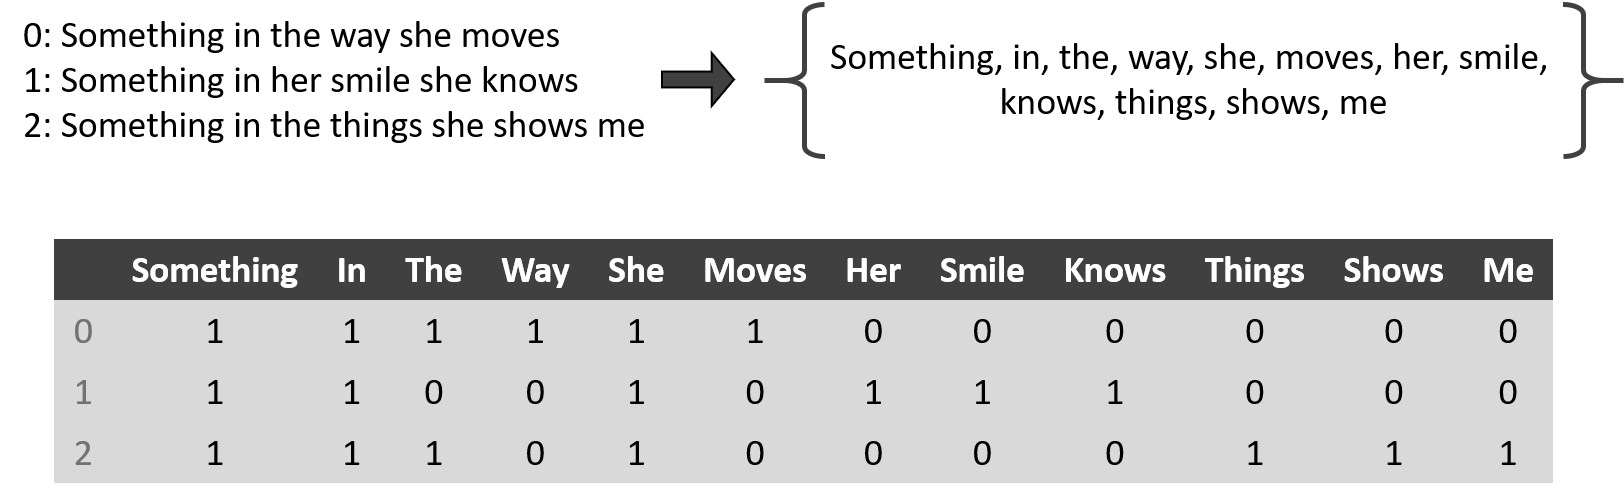
\includegraphics[width=\linewidth]{01.Chapters/02.Background/bag-of-words}
		\caption{Bag of Words example.}
		\label{fig:bag-of-words}
	\end{figure}
	
	\subsubsection{TF-IDF}
	
	Term Frequency Inverse Document Frequency, TF-IDF for short, it is applied to a BoW to determine the relative frequency for words in a specific document when compared to the inverse proportion of that word over all documents in the collection. So, it can be determined how important are the words in a specific document. 
	
	From BoW, for the $i^{\text{th}}$ vocabulary's word in the $j^{\text{th}}$ document, its TF-IDF weight is:
	
	\begin{equation}
	\label{eq:tf-idf}
	w_{i, j} = \text{tf}_{i, j} \times \log\left(\dfrac{N}{\text{df}_{i}}\right) \text{.}
	\end{equation}
	
	Where, the term frequency, $\text{tf}_{i, j}$, is how many time $i^{\text{th}}$ word appears in the $j^{\text{th}}$ document. The document frequency, $\text{df}_{i}$, is the number of documents in which th $i_{\text{th}}$ vocabulary words is present. And, finally, $N$ is the size of the document collection, with a large number of documents this term can explodes, so the logarithmic function is applied to dampen this effect.
	
	\subsection{Word Embedding}
	
	The vectorization methods such as BoW and TF-IDF can be very useful, but they can not represent the words context. This means that the same words used in different contexts have the same representation, just as different words used with the same meaning are represented differently. Besides that, an one-hot encoding method, like BoW, presents a very sparse representation with high dimensionality. 
	
	The Word Embedding is a technique to represent words in vectors capable of capture the words context in a document. It is also able to smooth the high dimensionality effect by using much more compact vector to represent the words.	
	
	There are three most know way to perform a good word embedding. We will describe briefly each one of them below. 
	
	\subsubsection{Word Representations in Vector Space} %word representations in vector space
	
	The first great word embedding technique emerged when Google researchers proposed two architectures to build continuous vector representations of words. Word's context can be observed as the words that surround it in a sentence. Then using shallow neural networks, it is possible to calculate the word vector space based on word's context, \cite{mikolov2013efficient}.
	
	The first suggested approach is the continuous bag of words or CBOW, the left side of Figure \ref{fig:word2vecarchitectures} show its architecture. Here the neural networks is designed to predict, given the context, which word is most likely to appear. So, words with the same probability to appear can have a shared dimension in the words vector space. 

	The second approach is known by Skip-Gram, architecture at right in Figure \ref{fig:word2vecarchitectures}. Very similar to CBOW, but instead of predicting the current word the Skip-Gram uses the current word as an input to a neural network to predict its context.
	
	\begin{figure}[h!]
		\centering
		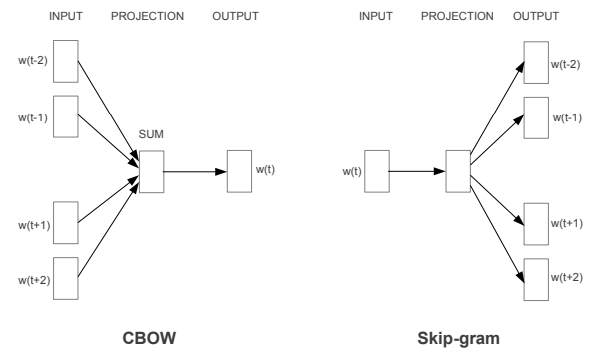
\includegraphics[width=0.85\linewidth]{01.Chapters/02.Background/word2vec_architectures}
		\caption{Word2Vec architectures \cite{mikolov2013efficient}.}
		\label{fig:word2vecarchitectures}
	\end{figure}
	
	% INCREMENTO: Explicar processo de treinamento, input/output e hidden layers
	
	After the network training process we can use the hidden layer weight matrix as an look up table to build the word embedding representation. The dimension for the vector space is managed by the number of neurons in the hidden layer. 		
	
	% INCREMENTO: Detalhes do artigo - base utilizada e testes
	
	\subsubsection{Global Vectors for Word Representation} % 
	
	Just a year later \citeonline{pennington-etal-2014-glove} arrives with a new approach to represent words in a vector space. The Global Vectors for Word Representation, or GloVe, method emerged by the need to consider some factors ignored by Skip-Gram.
		
	Methods such as Skip-Gram learn their embedding by targeting words to their respective context,
	ignoring the fact that some words appear more in a context than others. Thus, this co-occurrence of words only adds more useless training examples, increasing the training complexity without adding relevant information.
	
	GloVe, however, proposes to use the corpus statistics in a more efficient way. Using a weighted least squares model trained on a global word-word co-occurrence counts matrix. Thereby, it is possible to build a lookup table for the words in vocabulary and use it to represent them in a vector space.
	
	% INCREMENTO: Explicar processo de montagem das co-ocorrencias e probabilidades
	
	\subsubsection{Word Vectors with Subword Information}
		
	Both Skip-Gram and GloVe provide a good vector representation for words, but there still are an unsolved problem, What to do with unknown words? To solve this question was proposed a new embedding technique which uses subword units to build a vector space, \cite{bojanowski2017enriching}.
	
	Similar to Skip-Gram, this new method, the FastText, train its embedding by using a target to predict the context. However, instead of using the full words FastText goes a level deeper, breaking the words in $n$-grams, ie, the word becomes its own context. The Figure \ref{fig:apple-tri-gram} shows how the word ``apple'' can be broken into $n$-grams. 
		
	\begin{figure}[h!]
		\centering
		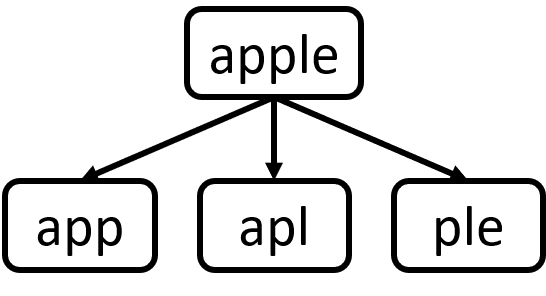
\includegraphics[width=0.3\linewidth]{01.Chapters/02.Background/apple-tri-gram}
		\caption{Tri-gram representation for ``apple'' word.}
		\label{fig:apple-tri-gram}
	\end{figure}
	
	There are a couple great advantages by using this method. It is now possible to generalize new words, or unseen in training data, since they have the same characters as known ones. Although it is possible to use available pre-trained models, the FastText requires less text to be trained, it can extract much more information from small pieces of text.	
	
	\subsection{Topic Clustering}
	
		
%	\subsection{Topic Classification}

\section{Machine Learning}

%\section{Deep Learning}
%	\subsection{Neuron}
%	\subsection{Perceptron and Activation Functions}
%	\subsection{Loss Functions}
%	\subsection{Optimization}
	
	